\documentclass{standalone}
\usepackage{tikz}
\usetikzlibrary{bbox}
\usetikzlibrary{calc}
\usetikzlibrary{arrows.meta,decorations.pathmorphing,backgrounds,positioning,fit,petri}

\def\centerarc[#1](#2)(#3:#4:#5)% Syntax: [draw options] (center) (initial angle:final angle:radius)
    { \draw[#1] ($(#2)+({#5*cos(#3)},{#5*sin(#3)})$) arc (#3:#4:#5); }

\begin{document}
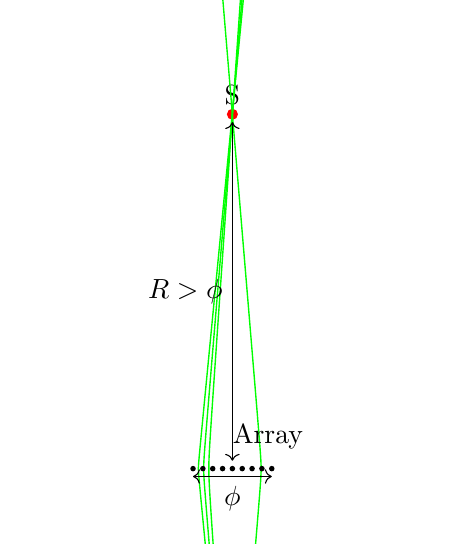
\begin{tikzpicture}
    [wave/.style={white!50!red,thick}]
    \coordinate[label={S}] (origin) at (0,2.5);
    \fill[red] (origin) circle (2pt);

    % \centerarc[wave](origin)(0:360:0.5)
    % \centerarc[wave](origin)(0:360:1)
    % \centerarc[wave](origin)(0:360:1.5)
    % \centerarc[wave](origin)(0:360:2.0)
    % \centerarc[wave](origin)(0:360:2.5)
    % \centerarc[wave](origin)(0:360:3)
    % \centerarc[wave](origin)(0:360:3.5)
    % \centerarc[wave](origin)(0:360:4)
    % \centerarc[wave](origin)(0:360:4.5)
    % \centerarc[wave](origin)(0:360:5.0)
    % \centerarc[wave](origin)(0:360:5.5)

    \def\tmax{5.6}
    \def\N{200}
    \def\a{0.006}
    \def\b{0.062}
    \draw[color=green,line width=0.5,samples=\N,variable=\t,domain=-\tmax:\tmax] % left
        plot({\a*cosh(\t) -7/16},{\b*sinh(\t) -2});
    
    \def\a{0.01037}
    \def\b{0.1245}
    \draw[color=green,line width=0.5,samples=\N,variable=\t,domain=-\tmax:\tmax] % left
        plot({\a*cosh(\t) -6/16},{\b*sinh(\t) -2});

    \def\a{0.013}
    \def\b{0.1870}
    \draw[color=green,line width=0.5,samples=\N,variable=\t,domain=-\tmax:\tmax] % left
        plot({\a*cosh(\t) -5/16},{\b*sinh(\t) -2});
    
    \def\a{-0.01037}
    \def\b{0.1245}
    \draw[color=green,line width=0.5,samples=\N,variable=\t,domain=-\tmax:\tmax] % left
        plot({\a*cosh(\t) + 6/16},{\b*sinh(\t) -2});

    \fill (-0.5,-2) circle (1pt);
    \fill (-3/8,-2) circle (1pt);
    \fill (-2/8,-2) circle (1pt);
    \fill (-1/8,-2) circle (1pt);
    \fill (-0.0,-2) circle (1pt);
    \fill (1/8,-2) circle (1pt);
    \fill (2/8,-2) circle (1pt);
    \fill (3/8,-2) circle (1pt);
    \fill (0.5,-2) circle (1pt);
    \node[label={Array}] at (0.45,-2) {};

    \draw [<->] (0,-1.9) -- (0,2.4) node[midway,left]{$R > \phi$};
    \draw [<->] (-0.5,-2.1) -- (0.5, -2.1) node[midway,below]{$\phi$};

    \pgfresetboundingbox
    \useasboundingbox(-2.6,-2.6)rectangle(2.6,3.6);
\end{tikzpicture}
\end{document}